\section{Results}\label{sec:results}

\begin{table}[t]
  \centering
  \caption{RQ1: Slices of the \numNPairs{} corpus-A pairs at $\ket{0\dots0}$. Wrong: slices that do not
  preserve the criterion (dynamic: of the \numNDynamicPairs{} pairs with measurement or feedback).
  Recall and precision are against the semantic dependences; size is the mean share of the circuit. Wire adds quantum dependence to the classical PDG; state-based pruning runs at $\ket{0\dots0}$.}
  \label{tab:rq1}
  \footnotesize\setlength{\tabcolsep}{3pt}
  \resizebox{\columnwidth}{!}{%
  \begin{tabular}{@{}l l r r r r r@{}}
    \toprule
    Rule & Dependence & Wrong & Dyn. & Recall & Prec. & Size \\
    \midrule
    Dependences$^{b}$  & semantic              & --                     & --                       & 1.000                 & 1.000                    & \numDepFloor{} \\
    \midrule
    Def-use            & data                  & \numRqOneDuUnsound{}   & \numDuDynamicUnsound{}   & \numRqOneDuRecall{}   & \numRqOneDuPrecision{}   & \numRqOneDuSize{} \\
    Classical PDG      & data, control         & \numCpdgUnsound{}      & \numCpdgDynamicUnsound{} & \numCpdgRecall{}      & \numCpdgPrecision{}      & \numCpdgSize{} \\
    Wire               & + quantum             & \numRqOneLcUnsound{}   & \numLcDynamicUnsound{}   & \numRqOneLcRecall{}   & \numRqOneLcPrecision{}   & \numRqOneLcSize{} \\
    QPDG reading       & wire + entangl.       & \numRqOneYzUnsound{}   & \numYzDynamicUnsound{}   & \numRqOneYzRecall{}   & \numRqOneYzPrecision{}   & \numRqOneYzSize{} \\
    \midrule
    Commutation$^{a}$  & wire, pruned          & \numLcqUnsound{}       & --                       & \numLcqRecall{}       & \numLcqPrecision{}       & \numLcqSize{} \\
    State-based        & wire, pruned          & \numRqOneQUnsound{}    & \numQDynamicUnsound{}    & \numRqOneQRecall{}    & \numRqOneQPrecision{}    & \numRqOneQSize{} \\
    \bottomrule
  \end{tabular}}\\[2pt]
  {\footnotesize $^{a}$\,On the \numLcqApplicable{} pairs where Qiskit's pass applies; it rejects
  circuits that measure, which leaves no dynamic pair. $^{b}$\,The semantic dependences themselves,
  the smallest dependence-complete slice. They are a reference, not a slicer, so they have no
  soundness value.}
\end{table}

\subsection{RQ1: Which definitions give sound and complete slices?}

Table~\ref{tab:rq1} shows that only the rules with quantum dependence are sound. The classical PDG gives a
wrong slice for \numCpdgUnsound{} of the \numNPairs{} pairs (\numCpdgUnsoundPct{}). Its control
dependence matters on circuits with measurement and feedback, where it is wrong on
\numCpdgDynamicUnsound{} pair against \numDuDynamicUnsound{} for def-use, which ignores classical bits. On
the unitary circuits the two rules are identical, and both are wrong on \numCpdgUnitaryUnsound{} pairs.
Of the dependences the classical PDG misses, \numCpdgMissKickback{} reach the criterion only through a
gate on which the criterion qubit is a control, the phase kickback of Proposition~\ref{prop:du}; only
\numCpdgMissFeedback{} reach it through classical feedback. The confirmatory test H1 confirms that
state-based pruning, which starts from the wire slice, is wrong on fewer pairs than def-use
(\numRqOneQUnsound{} against \numRqOneDuUnsound{}, exact McNemar, Holm \numHOnePHolm{}).

The wire rule is sound on every pair and recovers every dependence (recall \numRqOneLcRecall{}), as
Theorem~\ref{thm:sound} and Proposition~\ref{prop:complete} predict. Our reading of the quantum program
dependence graph is sound for the same reason, since its data edges already follow every qubit of a
gate, but its entanglement edges add operations that are not dependences. Its precision falls from
\numRqOneLcPrecision{} to \numRqOneYzPrecision{}, and its slices grow from \numRqOneLcSize{} to
\numRqOneYzSize{} of the circuit. On the \numFamCircuits{} circuits with known structure, no rule with
quantum dependence is ever wrong, while the classical PDG is wrong on \numFamCpdgUnsound{} of their
pairs. The \numCatEntries{} catalogue cases agree with the hand-derived expectations for every rule.

\begin{figure}[t]
  \centering
  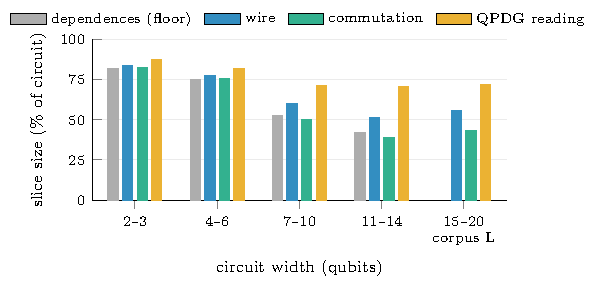
\includegraphics[width=\columnwidth]{figures/fig_size.pdf}
  \caption{RQ1: Mean slice size by circuit width. The grey bars are the dependences, the smallest size a
  dependence-complete slice can have. Corpus~L has no ground truth, which would need exact simulation of
  every perturbation at 15 to 20 qubits. Commutation is shown where Qiskit's pass applies.}
  \label{fig:size}
\end{figure}

Slice sizes should be read against the dependences themselves. The dependences of a qubit make up
\numDepFloor{} of its circuit on average, so no dependence-complete slice can be smaller, and the wire
slice keeps only \numLcExcess{} points more. It equals the dependence set exactly on \numLcExact{} of the
\numNPairs{} pairs, and on \numPairsAllDep{} pairs every operation of the circuit is a dependence. The
QPDG reading keeps \numYzExcess{} points more than the dependences. The sizes are large because most
benchmark circuits are small and densely coupled. Fig.~\ref{fig:size} shows that slices shrink as
circuits widen and less of a circuit can reach one qubit. At 11 to 14 qubits the wire slice keeps
\numWElevenLc{} of the circuit, and on the circuits of corpus~L it keeps \numCorpusLSizeLc{}. The QPDG
reading stays near \numCorpusLSizeYz{}, because entanglement closure links the operations of a whole
coupling component however wide the circuit is. Commutation falls below the floor, to \numWElevenLcq{} at
11 to 14 qubits. It is sound at the tested inputs but not dependence-complete. Deleting a gate that
commutes with the criterion's observables leaves the criterion unchanged, although a different gate at
the same position would change it.

\subsection{RQ2: How much precision beyond the wire slice is safe?}

\begin{figure}[t]
  \centering
  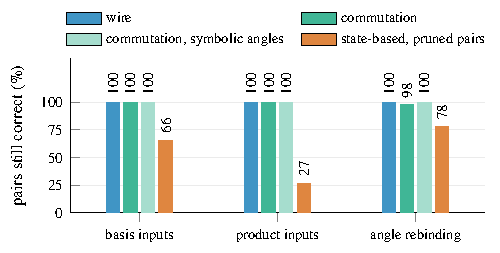
\includegraphics[width=\columnwidth]{figures/fig_robust.pdf}
  \caption{RQ2: Share of pairs whose slice, computed at $\ket{0\dots0}$, stays correct in all
  \numRobDraws{} draws of each input regime. State-based pruning is shown for the
  \numHThreePrunedN{} pairs it prunes; on the others it equals the wire slice.}
  \label{fig:robust}
\end{figure}

Both refinements make slices smaller, but only commutation keeps them correct. State-based pruning
shrinks the wire slice by \numHTwoDiff{} percentage points of the circuit (95\% CI \numHTwoCILow{} to
\numHTwoCIHigh{}), a relative reduction of \numHTwoRelative{}, and is smaller on \numHTwoSmaller{} pairs
(H2, Wilcoxon, Holm \numHTwoPHolm{}). Fig.~\ref{fig:robust} shows what that costs. Of the pairs it
prunes, the slice stays correct for all random product inputs on only \numHThreePrunedRate{}, and over
all pairs on \numHThreeRate{} (Wilson CI \numHThreeCILow{} to \numHThreeCIHigh{}), far below the
pre-registered threshold of 95\% (H3 fails). State-based pruning is therefore a property of one input,
not of the program.

Commutation is smaller than the wire slice on \numLcqSmallerThanLc{} of \numLcqApplicable{} pairs and
stays correct on every random basis and product input. It fails only when the angles change, on
\numRobLcqParamFail{} pairs of variational circuits whose gates commute with the
criterion's observable at their written angle. State-based pruning is only \numQVsLcqReduction{} smaller
than commutation on average, and larger on \numQLargerThanLcq{} pairs. Commutation also misses
dependences (recall \numLcqRecall{}). It drops a gate that commutes with the observable, although a fault
at that gate could still change the criterion.

\subsection{RQ3: What does each definition do to fault localization?}

The wire slice of the faulty circuit contains the fault site in \numRqThreeContainLc{} of the
\numRqThreeUnits{} units, against \numRqThreeContainCpdg{} for the classical PDG,
\numRqThreeContainQ{} for state-based pruning, and \numRqThreeContainRandom{} for a random set of the
state-based slice's size. All \numLcMissTotal{} units the wire slice misses are omission faults, a
removed control (\numLcMissCrm{}), a re-targeted operand (\numLcMissQsw{}), a removed preparation of an
entangling gate (\numLcMissEnt{}) or a deleted gate (\numLcMissDel{}). These faults delete the interaction
that a slice of the faulty program would have to follow, a limit of slicing any faulty program rather
than of the rule.

State-based pruning loses \numHFourLoss{} percentage points of containment against the wire slice
(CI \numHFourCILow{} to \numHFourCIHigh{}), so H4, which allowed a loss of at most five points, fails. In
\numCQFour{} units the wire slice contains the fault and the pruned slice does not. In most of them the
fault makes the criterion separable from qubits it should be correlated with, and pruning then removes the
faulty operation as irrelevant to the single criterion qubit. Slicing with a criterion over all the wrong
qubits recovers \numCQFourRecovered{} of these units. The pruned slices are smaller where both contain the
fault, by \numHFiveSizeDiff{} instructions on average (H5), but the fault then ranks later within them
(EXAM difference \numHFiveExamDiff{}). Mutation-based fault localization confirms that pruning does not
help a ranking. Its mean EXAM score is \numMbflExamAll{} over the whole circuit, \numMbflExamLc{} within
the wire slice and \numMbflExamQ{} within the state-based slice (lower is better).

\begin{figure}[t]
  \centering
  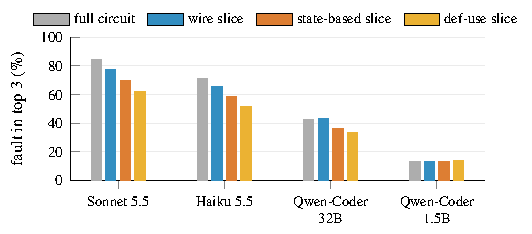
\includegraphics[width=\columnwidth]{figures/fig_llm.pdf}
  \caption{RQ3: Share of the \numTTwoItems{} faulty circuits for which a language model names the faulty
  instruction among its top three, given the whole circuit or a slice of it.}
  \label{fig:llm}
\end{figure}

Language models localize faults worse from pruned slices (Fig.~\ref{fig:llm}). Claude Sonnet~5.5 finds
the fault in its top three for \numTTwoSonnetFull{} of the faulty circuits, \numTTwoSonnetLc{} of the wire
slices and \numTTwoSonnetQ{} of the state-based slices. The state-based slice is
\numTTwoMaxDrop{} points worse than the full circuit (CI \numTTwoSonnetQVsFullCI{}, exact McNemar
\numTTwoSonnetQVsFullP{}) and \numTTwoSonnetQVsLcLoss{} points worse than the wire slice
(\numTTwoSonnetQVsLcP{}). Haiku~5.5 and Qwen2.5-Coder-32B show the same order, and the 1.5B model
localizes too few faults for the input to matter. No slice beats the whole circuit for these models.
Slicing does not hand a model information it lacks; it can only remove the fault.

On the real Bugs4Q programs, the wire slices keep every faulty line, as do the full programs, while
removing little, \numLinesLcMean{} of \numLinesFullMean{} lines on average over \numLinesUnits{} units.
These programs are small. Def-use loses the faulty line in one unit, the bug of
Section~\ref{sec:example}. An independent mapping by the authors' static Qiskit parser agrees with ours
on all \numMapCrossAgree{} instructions both could map.

\subsection{RQ4: What does it cost?}

\begin{figure}[t]
  \centering
  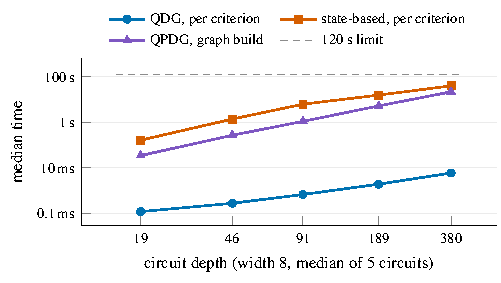
\includegraphics[width=\columnwidth]{figures/fig_cost.pdf}
  \caption{RQ4: Median time per criterion and of building the dependence graph, for circuits of width 8
  and growing depth. At the two largest depths, only the criteria finished within the limit are counted,
  so the state-based time is a lower bound.}
  \label{fig:cost}
\end{figure}

The wire slice costs milliseconds at every depth (Fig.~\ref{fig:cost}), at most \numCostLcMaxMs{}~ms per
circuit. State-based pruning simulates the circuit for every candidate removal. Its time grows with depth
and exceeds the \numCostWallLimit{}~s limit for \numCostDepthEightyOverLimit{} of the 5 circuits at the
second-largest depth and for all \numCostDepthOneSixtyOverLimit{} at the largest. It also grows
exponentially with width, reaching \numCostWidthQMax{}~s at 14 qubits. On corpus~L it completes on
\numCorpusLCompleted{} of \numCorpusLCircuits{} circuits of 15 to 20 qubits. A graph with entanglement
edges is itself costly, because the closure links every pair of operations on a coupling component; the
wire rule needs only the per-qubit edges.
